\section{ECKA}
\begin{frame}{ECKA}
    \begin{figure}[!htb]
        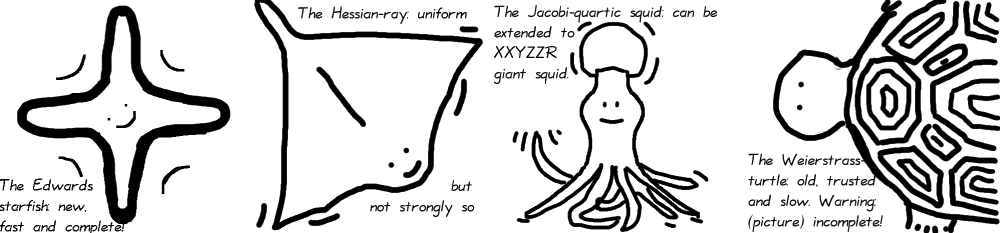
\includegraphics[height=25mm]{data/ec-types.png}
    \end{figure}
    \begin{figure}[!htb]
        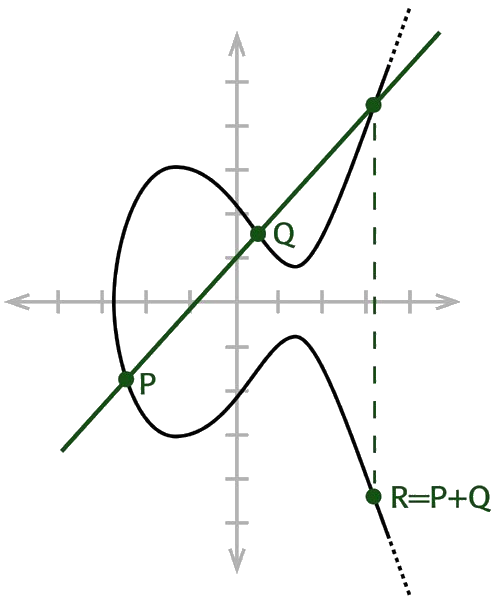
\includegraphics[height=25mm]{data/ec.png}\hspace{10mm}
        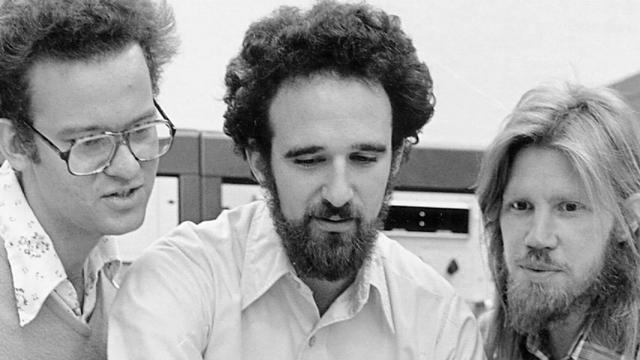
\includegraphics[height=25mm]{data/merkle-hellman-diffie.jpg}\hspace{10mm}
        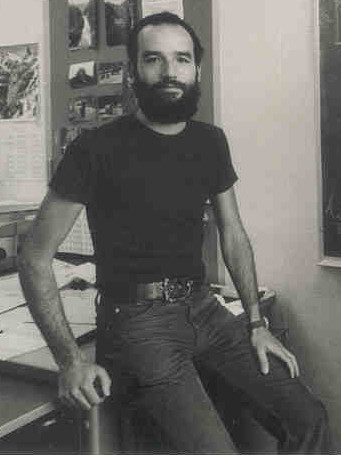
\includegraphics[height=25mm]{data/shamir.jpg}
    \end{figure}
\end{frame}

\subsection{Challenge}
\begin{frame}{Story}{Infos}
    \begin{itemize}
        \item Service using key agreement on elliptic curves
        \item Combines two different ones: \begin{enumerate}
           \item Exchange a point P
           \item Agree on key
           \item Send AES-ECB encrypted password
        \end{enumerate}
    \end{itemize}
    Hint: He, we have the latest news for you.
    The first part of their strange key agreement
    was designed by the famous SHA-Robot \textsc{Mir}!
\end{frame}

\begin{frame}{Stats}
    \begin{itemize}
        \item Category: Crypto
        \item Points: 100
        \item Solved by: 5 Teams
    \end{itemize}
\end{frame}

\subsection{Service}
\begin{frame}{Service}
    \begin{figure}[!htb]
        
\includegraphics[height=45mm]{data/demo.png}
    \end{figure}
\end{frame}

\subsection{Crypto Stuff}
\begin{frame}{Crypto Stuff}
    Involved Crypto-Stuff
    \begin{itemize}
        \item Elliptic Curve Crypto (ECC)
        \item Key Agreements: \begin{itemize}
            \item ThreePass
            \item Diffie Hellman
        \end{itemize}
    \end{itemize}
\end{frame}
\begin{frame}{ECC}{Elliptic Curve Cryptography}
    \begin{itemize}
        \item asymmetric crypto
        \item uses elliptic curves over finite fields as group
        \item thus can replace other groups (normally $\mathbb{Z}_p^*$)
        \item good properties like small key size etc.
    \end{itemize}
    \begin{itemize}
        \item Discrete Logarithm Problem (DLP) is hard
        \item algorithms like DHKE, Elgamal can be used
    \end{itemize}
\end{frame}

\begin{frame}{ThreePass}{on Elliptic Curves}
\begin{figure}[!htb]
    \begin{protocol}{2}
    \protocolheader{$\mathcal{E}(\mathbb{Z}_p^*)$}
    \participants{\textbf{Alice}}{\textbf{Bob}}\\ 
        \doesA{$\alpha \in_R \mathbb{Z}_p^*$}
        \doesA{$P \in \mathcal{E}(\mathbb{Z}_p^*)$}
        \doesA{$P_{\alpha} = \alpha P$}
        & \sends{P_{\alpha}} & \\[-5mm]
        \doesB{$\beta \in_R \mathbb{Z}_p^*$}
        \doesB{$P_{\alpha\beta} = \beta P_{\alpha}$}
        &\receives{P_{\alpha\beta}} & \\[-5mm]
        \doesA{$P_{\beta}=\alpha^{-1}\cdot P_{\alpha\beta}$}
        & \sends{P_{\beta}} & \\[-5mm]
        \doesB{$P=\beta^{-1}\cdot P_{\beta}$}
    \end{protocol}
\end{figure}
\end{frame}

\begin{frame}{DHKE}{on Elliptic Curves}
\begin{figure}[!htb]
    \begin{protocol}{2}
    \protocolheader{$\mathcal{E}(\mathbb{Z}_p^*),\,P \in \mathcal{E}(\mathbb{Z}_p^*)$}
    \participants{\textbf{Alice}}{\textbf{Bob}}\\ 
        \doesA{$\alpha \in_R \mathbb{Z}_p^*$}
        \doesA{$P_{\alpha} = \alpha P$}
        & \sends{P_{\alpha}} & \\[-5mm]
        \doesB{$\beta \in_R \mathbb{Z}_p^*$}
        \doesB{$P_{\beta} = \beta P$}
        &\receives{P_{\beta}} & \\[-5mm]
        \doesA{$P_{\alpha \beta}=\alpha \cdot P_{\beta}$}
        \doesB{$P_{\alpha \beta}=\beta \cdot P_{\alpha}$}
    \end{protocol}
\end{figure}
\end{frame}

\subsection{Solution}
\begin{frame}{Solution}
    \begin{figure}[!htb]
        
\includegraphics[height=45mm]{data/demo.png}
    \end{figure}
\end{frame}
